\subsection{The Averaging Law}
Fig.~\ref{fig:averaging} tests \eqref{eq:pred} within participants, with the prediction for every $k>1$ computed from the observed single-trial accuracy alone. For N170, N400, and N2pc the predicted curve runs inside the 95\% interval of the observed curve at every $k$. N400 rises from 0.538 at $k=1$ to 0.595 at $k=8$ against a prediction of 0.607, and N2pc from 0.506 to 0.530 at $k=16$. MMN starts at 0.500, where $\Phi^{-1}(\BA(1))=0$, and the law predicts no growth. The observed curve stays between 0.498 and 0.503 for all $k$, an internal control whose brief, sign-changing difference barely moves the epoch mean. P3 rises faster than predicted, reaching 0.538 at $k=4$ against 0.509. Its single-trial estimate, 0.504, lies where $\Phi^{-1}$ amplifies sampling error, and its rare condition supports averages up to $k=4$. Under pre-stimulus scaling every paradigm stays within 0.489 to 0.507 for every $k$.

\begin{figure*}[t]
\centering
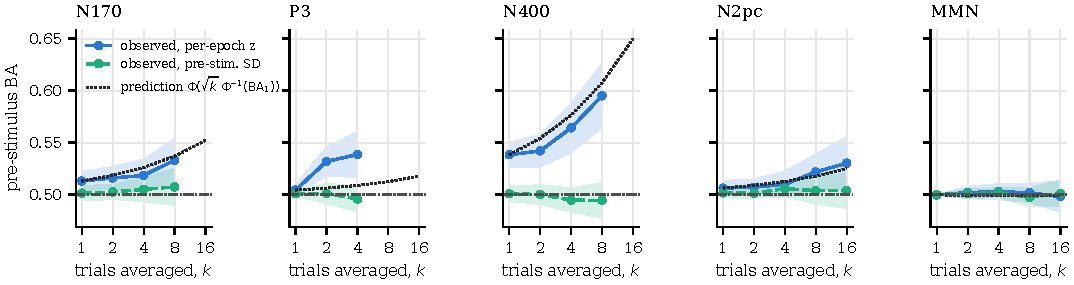
\includegraphics[width=\textwidth]{figures/fig_averaging.pdf}
\caption{The averaging law on ERP CORE, within participants. Pre-stimulus decoding of pseudo-trials averaged over $k$ trials, mean and 95\% interval over participants. Dotted: the prediction $\Phi(\sqrt{k}\,\Phi^{-1}(\BA_1))$ computed from the observed $k=1$ value alone. P3 stops at $k=4$ because its rare condition has too few trials per fold.}
\label{fig:averaging}
\end{figure*}
